\documentclass[14pt]{extbook}
\usepackage{multicol, enumerate, enumitem, hyperref, color, soul, setspace, parskip, fancyhdr} %General Packages
\usepackage{amssymb, amsthm, amsmath, latexsym, units, mathtools} %Math Packages
\everymath{\displaystyle} %All math in Display Style
% Packages with additional options
\usepackage[headsep=0.5cm,headheight=12pt, left=1 in,right= 1 in,top= 1 in,bottom= 1 in]{geometry}
\usepackage[usenames,dvipsnames]{xcolor}
\usepackage{dashrule}  % Package to use the command below to create lines between items
\newcommand{\litem}[1]{\item#1\hspace*{-1cm}\rule{\textwidth}{0.4pt}}
\pagestyle{fancy}
\lhead{Progress Quiz 10}
\chead{}
\rhead{Version B}
\lfoot{5170-5105}
\cfoot{}
\rfoot{Summer C 2021}
\begin{document}

\begin{enumerate}
\litem{
Solve the quadratic equation below. Then, choose the intervals that the solutions belong to, with $x_1 \leq x_2$ (if they exist).\[ 19x^{2} -15 x + 2 = 0 \]\begin{enumerate}[label=\Alph*.]
\item \( x_1 \in [2.86, 3.71] \text{ and } x_2 \in [11.49, 13.24] \)
\item \( x_1 \in [-1.4, -0.06] \text{ and } x_2 \in [-0.47, 0.17] \)
\item \( x_1 \in [-0.2, 0.26] \text{ and } x_2 \in [0.42, 0.63] \)
\item \( x_1 \in [-8.47, -7.98] \text{ and } x_2 \in [8.44, 9.67] \)
\item \( \text{There are no Real solutions.} \)

\end{enumerate} }
\litem{
Solve the quadratic equation below. Then, choose the intervals that the solutions $x_1$ and $x_2$ belong to, with $x_1 \leq x_2$.\[ 25x^{2} -10 x -24 = 0 \]\begin{enumerate}[label=\Alph*.]
\item \( x_1 \in [-20.67, -19.77] \text{ and } x_2 \in [29.7, 30.12] \)
\item \( x_1 \in [-1.68, -1.44] \text{ and } x_2 \in [0.34, 0.8] \)
\item \( x_1 \in [-1.02, -0.6] \text{ and } x_2 \in [1.04, 1.54] \)
\item \( x_1 \in [-4.46, -3.87] \text{ and } x_2 \in [0.15, 0.31] \)
\item \( x_1 \in [-0.54, 0] \text{ and } x_2 \in [2.39, 2.52] \)

\end{enumerate} }
\litem{
Graph the equation below.\[ f(x) = -(x+4)^2 + 20 \]\begin{enumerate}[label=\Alph*.]
\begin{multicols}{2}\item 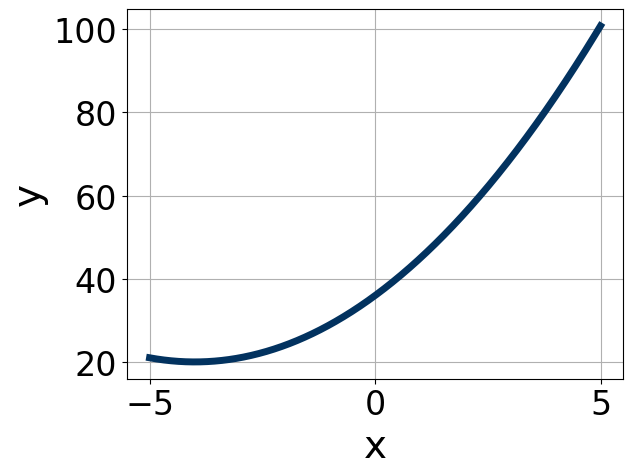
\includegraphics[width = 0.3\textwidth]{../Figures/quadraticEquationToGraphAB.png}\item 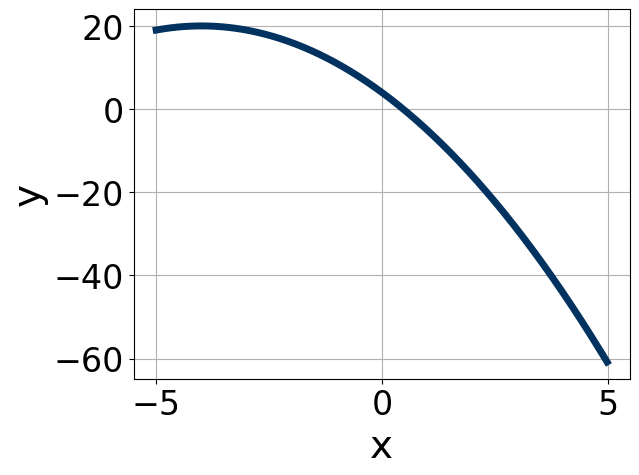
\includegraphics[width = 0.3\textwidth]{../Figures/quadraticEquationToGraphBB.png}\item 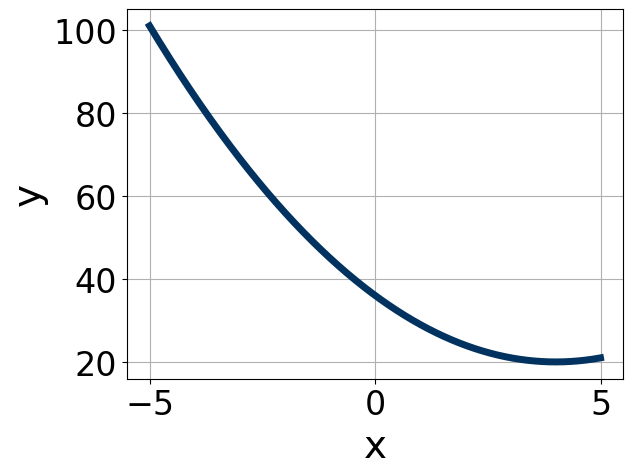
\includegraphics[width = 0.3\textwidth]{../Figures/quadraticEquationToGraphCB.png}\item 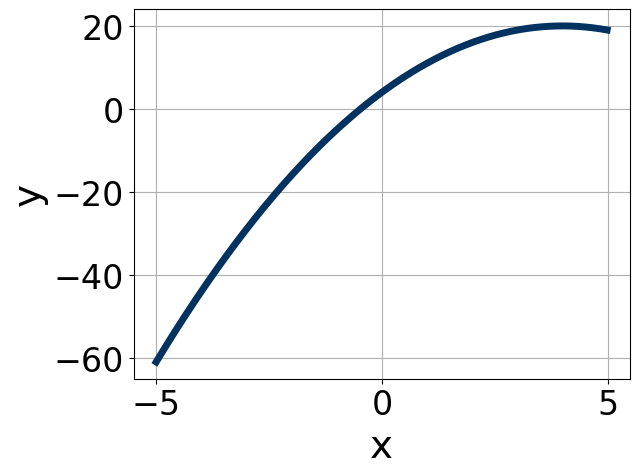
\includegraphics[width = 0.3\textwidth]{../Figures/quadraticEquationToGraphDB.png}\end{multicols}\item None of the above.
\end{enumerate} }
\litem{
Write the equation of the graph presented below in the form $f(x)=ax^2+bx+c$, assuming  $a=1$ or $a=-1$. Then, choose the intervals that $a, b,$ and $c$ belong to.
\begin{center}
    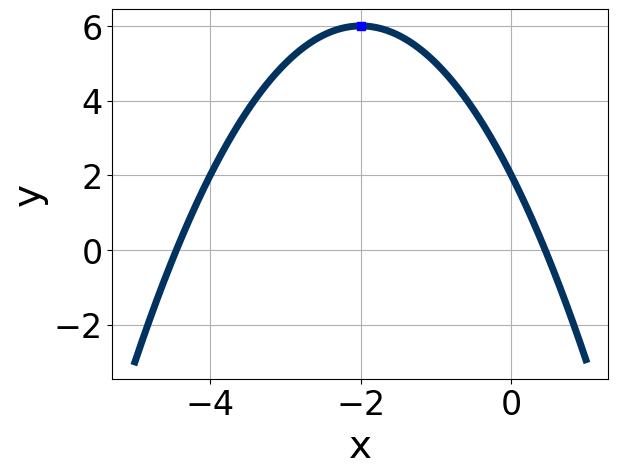
\includegraphics[width=0.5\textwidth]{../Figures/quadraticGraphToEquationB.png}
\end{center}
\begin{enumerate}[label=\Alph*.]
\item \( a \in [0.4, 1.1], \hspace*{5mm} b \in [3, 6], \text{ and } \hspace*{5mm} c \in [8, 11] \)
\item \( a \in [-2.2, -0.7], \hspace*{5mm} b \in [3, 6], \text{ and } \hspace*{5mm} c \in [1, 3] \)
\item \( a \in [-2.2, -0.7], \hspace*{5mm} b \in [3, 6], \text{ and } \hspace*{5mm} c \in [-11, -7] \)
\item \( a \in [-2.2, -0.7], \hspace*{5mm} b \in [-6, -2], \text{ and } \hspace*{5mm} c \in [1, 3] \)
\item \( a \in [0.4, 1.1], \hspace*{5mm} b \in [-6, -2], \text{ and } \hspace*{5mm} c \in [8, 11] \)

\end{enumerate} }
\litem{
Factor the quadratic below. Then, choose the intervals that contain the constants in the form $(ax+b)(cx+d); b \leq d.$\[ 24x^{2} +2 x -15 \]\begin{enumerate}[label=\Alph*.]
\item \( a \in [-1.4, 3.3], \hspace*{5mm} b \in [-5, 2], \hspace*{5mm} c \in [17.7, 19.4], \text{ and } \hspace*{5mm} d \in [5, 7] \)
\item \( a \in [-1.4, 3.3], \hspace*{5mm} b \in [-21, -16], \hspace*{5mm} c \in [0.7, 1.8], \text{ and } \hspace*{5mm} d \in [16, 26] \)
\item \( a \in [2.5, 5.6], \hspace*{5mm} b \in [-5, 2], \hspace*{5mm} c \in [3.7, 6.9], \text{ and } \hspace*{5mm} d \in [5, 7] \)
\item \( a \in [6.2, 8.5], \hspace*{5mm} b \in [-5, 2], \hspace*{5mm} c \in [2.2, 3.4], \text{ and } \hspace*{5mm} d \in [5, 7] \)
\item \( \text{None of the above.} \)

\end{enumerate} }
\litem{
Solve the quadratic equation below. Then, choose the intervals that the solutions $x_1$ and $x_2$ belong to, with $x_1 \leq x_2$.\[ 25x^{2} +60 x + 36 = 0 \]\begin{enumerate}[label=\Alph*.]
\item \( x_1 \in [-31.73, -29.14] \text{ and } x_2 \in [-30.24, -29.98] \)
\item \( x_1 \in [-1.73, -0.47] \text{ and } x_2 \in [-1.36, -1.08] \)
\item \( x_1 \in [-7.85, -5.72] \text{ and } x_2 \in [-0.24, -0.19] \)
\item \( x_1 \in [-4.58, -3] \text{ and } x_2 \in [-0.56, -0.37] \)
\item \( x_1 \in [-3.3, -2.28] \text{ and } x_2 \in [-0.64, -0.54] \)

\end{enumerate} }
\litem{
Write the equation of the graph presented below in the form $f(x)=ax^2+bx+c$, assuming  $a=1$ or $a=-1$. Then, choose the intervals that $a, b,$ and $c$ belong to.
\begin{center}
    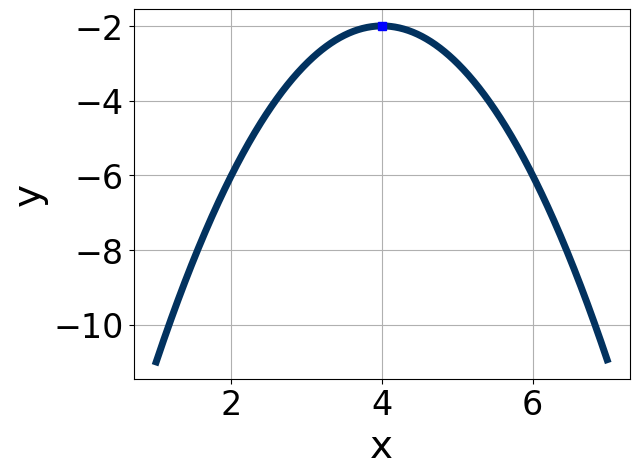
\includegraphics[width=0.5\textwidth]{../Figures/quadraticGraphToEquationCopyB.png}
\end{center}
\begin{enumerate}[label=\Alph*.]
\item \( a \in [-1.6, -0.3], \hspace*{5mm} b \in [-11, -7], \text{ and } \hspace*{5mm} c \in [-16, -12] \)
\item \( a \in [-1.6, -0.3], \hspace*{5mm} b \in [7, 10], \text{ and } \hspace*{5mm} c \in [-18, -16] \)
\item \( a \in [-0.2, 1.4], \hspace*{5mm} b \in [-11, -7], \text{ and } \hspace*{5mm} c \in [13, 16] \)
\item \( a \in [-0.2, 1.4], \hspace*{5mm} b \in [7, 10], \text{ and } \hspace*{5mm} c \in [13, 16] \)
\item \( a \in [-1.6, -0.3], \hspace*{5mm} b \in [-11, -7], \text{ and } \hspace*{5mm} c \in [-18, -16] \)

\end{enumerate} }
\litem{
Solve the quadratic equation below. Then, choose the intervals that the solutions belong to, with $x_1 \leq x_2$ (if they exist).\[ 13x^{2} +10 x -4 = 0 \]\begin{enumerate}[label=\Alph*.]
\item \( x_1 \in [-0.39, 0.11] \text{ and } x_2 \in [1.03, 1.41] \)
\item \( x_1 \in [-1.3, -0.98] \text{ and } x_2 \in [0.07, 0.31] \)
\item \( x_1 \in [-19.67, -16.86] \text{ and } x_2 \in [16.94, 17.17] \)
\item \( x_1 \in [-14.27, -13.31] \text{ and } x_2 \in [3.72, 3.78] \)
\item \( \text{There are no Real solutions.} \)

\end{enumerate} }
\litem{
Factor the quadratic below. Then, choose the intervals that contain the constants in the form $(ax+b)(cx+d); b \leq d.$\[ 24x^{2} -2 x -15 \]\begin{enumerate}[label=\Alph*.]
\item \( a \in [8.8, 13], \hspace*{5mm} b \in [-6, -3], \hspace*{5mm} c \in [1.98, 3.21], \text{ and } \hspace*{5mm} d \in [3, 11] \)
\item \( a \in [2.4, 4], \hspace*{5mm} b \in [-6, -3], \hspace*{5mm} c \in [7.53, 8.05], \text{ and } \hspace*{5mm} d \in [3, 11] \)
\item \( a \in [4.1, 7.5], \hspace*{5mm} b \in [-6, -3], \hspace*{5mm} c \in [3.91, 4.62], \text{ and } \hspace*{5mm} d \in [3, 11] \)
\item \( a \in [-0.1, 2.2], \hspace*{5mm} b \in [-24, -14], \hspace*{5mm} c \in [0.85, 1], \text{ and } \hspace*{5mm} d \in [15, 25] \)
\item \( \text{None of the above.} \)

\end{enumerate} }
\litem{
Graph the equation below.\[ f(x) = (x-2)^2 + 17 \]\begin{enumerate}[label=\Alph*.]
\begin{multicols}{2}\item 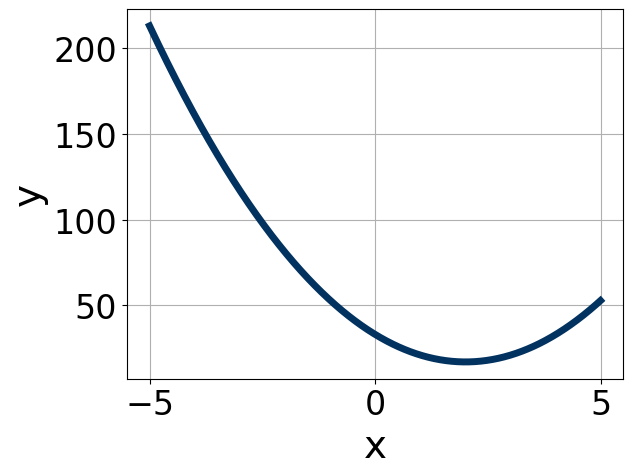
\includegraphics[width = 0.3\textwidth]{../Figures/quadraticEquationToGraphCopyAB.png}\item 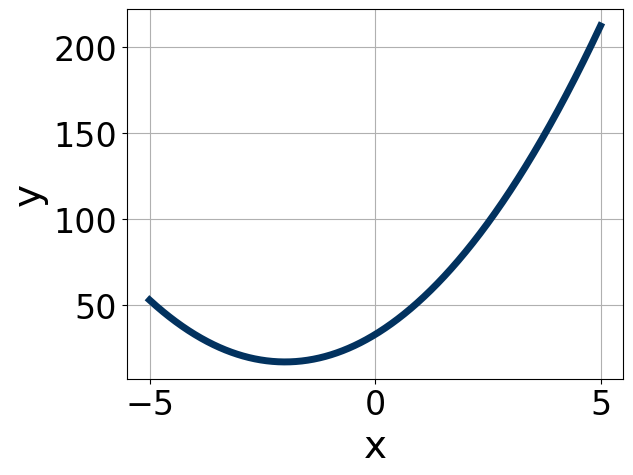
\includegraphics[width = 0.3\textwidth]{../Figures/quadraticEquationToGraphCopyBB.png}\item 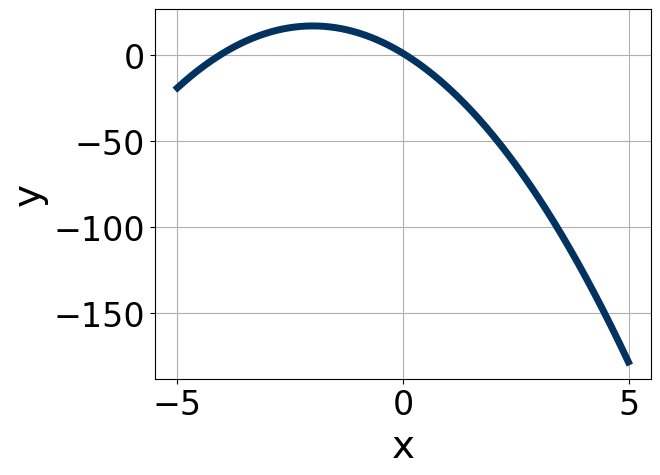
\includegraphics[width = 0.3\textwidth]{../Figures/quadraticEquationToGraphCopyCB.png}\item 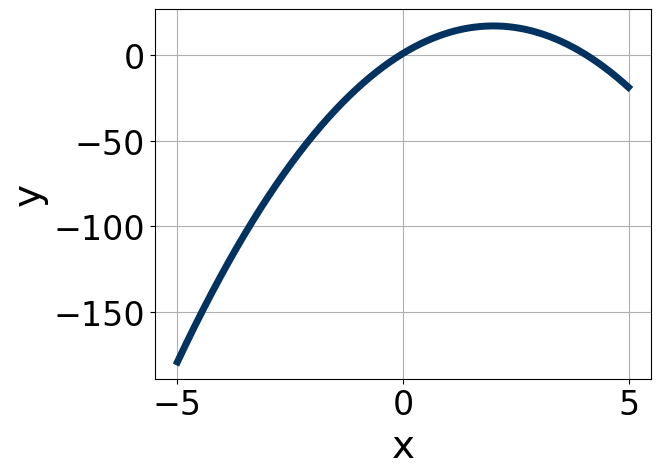
\includegraphics[width = 0.3\textwidth]{../Figures/quadraticEquationToGraphCopyDB.png}\end{multicols}\item None of the above.
\end{enumerate} }
\end{enumerate}

\end{document}